\documentclass[tikz,border=2pt]{standalone}
\usepackage{amsmath}
\usepackage{amssymb}
\usepackage{xcolor}

\definecolor{journalink}{HTML}{1F1C18}
\definecolor{journalmuted}{HTML}{8A7F72}
\definecolor{journalaccent}{HTML}{9C2D2D}

% #1 = row y, #2 = row label
\newcommand{\axisrow}[2]{%
  \draw[journalink, line width=0.8pt, ->, >=stealth] (0,#1) -- (6.0,#1);
  \node[journalink, right] at (6.0,#1) {#2};
  \draw[journalink, line width=0.8pt] (1.2,{#1+0.16}) -- (1.2,{#1-0.16});
  \node[journalink, below, font=\small] at (1.2,{#1-0.16}) {$0$};
  \draw[journalink, line width=0.8pt] (5.0,{#1+0.16}) -- (5.0,{#1-0.16});
  \node[journalink, below, font=\small] at (5.0,{#1-0.16}) {$1$};
}
\newcommand{\segrow}[3]{\draw[journalaccent, line width=1.8pt] (#2,#1) -- (#3,#1);}
\newcommand{\closeddot}[2]{\fill[journalink] (#2,#1) circle (2.2pt);}

\begin{document}
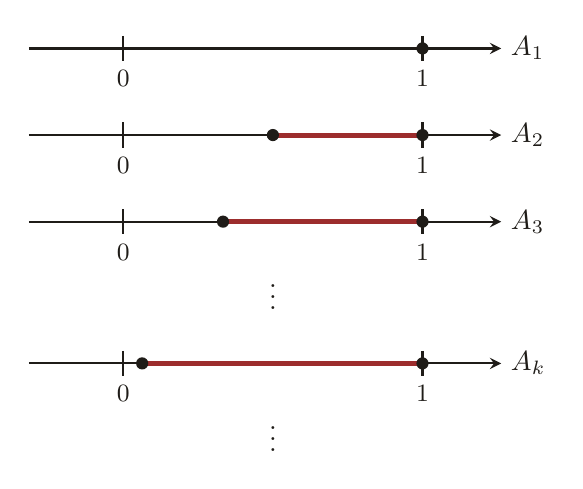
\begin{tikzpicture}[x=1cm, y=1cm, every node/.style={font=\normalsize}]

  \axisrow{0}{$A_1$}
  \closeddot{0}{5.0}

  \axisrow{-1.1}{$A_2$}
  \segrow{-1.1}{3.1}{5.0}
  \closeddot{-1.1}{3.1}
  \closeddot{-1.1}{5.0}

  \axisrow{-2.2}{$A_3$}
  \segrow{-2.2}{2.467}{5.0}
  \closeddot{-2.2}{2.467}
  \closeddot{-2.2}{5.0}

  \node[journalink] at (3.1,-3.05) {$\vdots$};

  \axisrow{-4.0}{$A_k$}
  \segrow{-4.0}{1.44}{5.0}
  \closeddot{-4.0}{1.44}
  \closeddot{-4.0}{5.0}

  \node[journalink] at (3.1,-4.85) {$\vdots$};

\end{tikzpicture}
\end{document}
